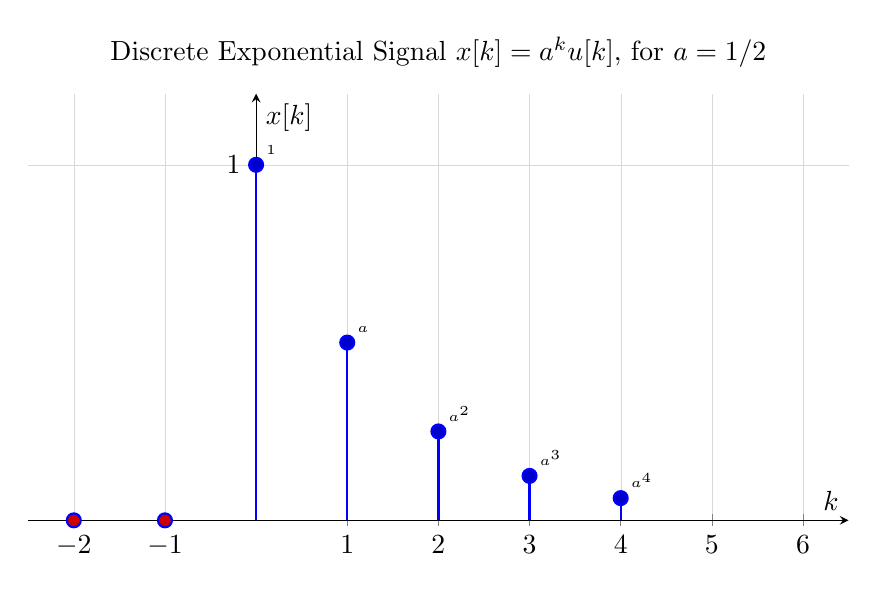
\begin{tikzpicture}
	\pgfplotsset{impulse/.style={ycomb,blue,thick,mark=*,mark size=2.5pt}}
	\begin{axis}[
		width=12cm,
		height=7cm,
		title={Discrete Exponential Signal $x[k] = a^k u[k]$, for $a=1/2$},
		xlabel={$k$},
		ylabel={$x[k]$},
		axis lines=middle,
		xmin=-2.5, xmax=6.5,
		ymin=0, ymax=1.2,
		xtick={-2,-1,0,1,2,3,4,5,6},
		ytick={1},
		grid=major,
		grid style={line width=.1pt, draw=gray!30},
		]
		\addplot+[impulse,nodes near coords,point meta=explicit symbolic,
		every node near coord/.style={anchor=south west,font=\tiny,text=black}] 
		table [meta=label] {
			x y label
			0 1 {$1$}
			1 0.5 {$a$}
			2 0.25 {$a^2$}
			3 0.125 {$a^3$}
			4 0.0625 {$a^4$}
		};
		\addplot+[impulse] coordinates {(-2,0)(-1,0)};
	\end{axis}
\end{tikzpicture}